\section{UML MODELS}
\subsection{Use case diagram}
\subsection{Use case Description and sequence diagram}
\subsubsection{Registation}
\begin {tabular} {|p{3cm}|p{10cm}|}
\hline
Goal & G1\\
\hline
Actor & Guest\\
\hline
Entry conditions & None\\
\hline
Flow of events &
\begin {itemize}
\item The guest enters the website
\item The guest clicks the registration button
\item The guest fills the registrationo form
\item The Guest clicks on CONFIRM button
\end {itemize}\\
\hline
Exit conditions & The system shows the home page to the user and updates its database.\\
\hline
Exceptions & The email is already registered in the system or some fields are empty.\\
\hline
\end {tabular}
\begin{figure}[h!]
	\centering
%	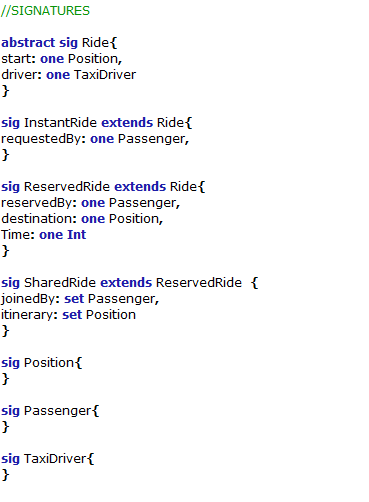
\includegraphics[height=0.75\textwidth]{Sig}
\end{figure}
\newpage

\subsubsection{Login}
\begin {tabular} {|p{3cm}|p{10cm}|}
\hline
Goal & G2\\
\hline
Actor & Guest\\
\hline
Entry conditions & none\\
\hline
Flow of events &
\begin {itemize}
\item The guest enters the website
\item The guest fills the fields Username/Password
\item The Guest clicks on login button
\end {itemize}\\
\hline
Exit conditions & The system shows the personal page to the user.\\
\hline
Exceptions & Username and password combination is invalid.\\
\hline
\end {tabular}
\begin{figure}[h!]
	\centering
	%	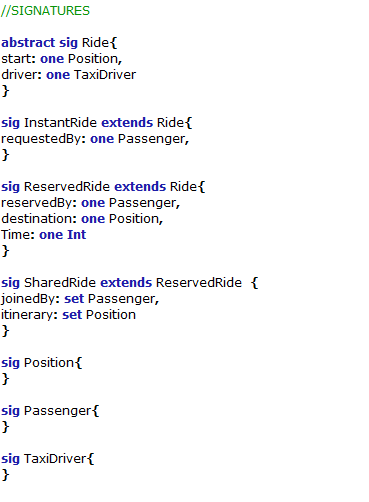
\includegraphics[height=0.75\textwidth]{Sig}
\end{figure}
\newpage

\subsubsection{Request ride}
\begin {tabular} {|p{3cm}|p{10cm}|}
\hline
Goal & G3 \\
\hline
Actor & Passenger\\
\hline
Entry conditions & User registered and logged in\\
\hline
Flow of events &
\begin {itemize}
\item The passenger clicks on request button
\item The passenger insert his current location in the apposite field
\item The passenger clicks on confirm button
\end {itemize}\\
\hline
Exit conditions & The system find a taxi and send a confirmation to the user.\\
\hline
Exceptions & Location provided by the user is invalid\\
\hline
\end {tabular}
\begin{figure}[h!]
	\centering
	%	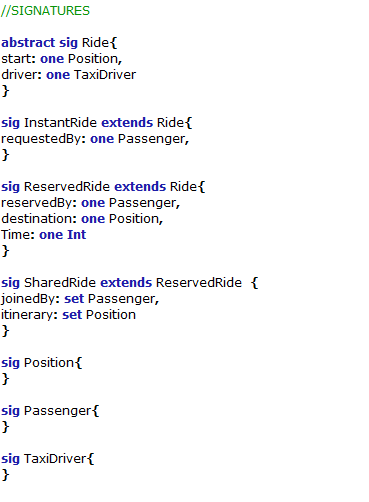
\includegraphics[height=0.75\textwidth]{Sig}
\end{figure}
\newpage

\subsubsection{Reserve a ride}
\begin {tabular} {|p{3cm}|p{10cm}|}
\hline
Goal & G4\\
\hline
Actor & Passenger\\
\hline
Entry conditions & User registered and logged in\\
\hline
Flow of events &
\begin {itemize}
\item The passenger clicks on reservation button
\item The passenger insert his current location, destination and time of the ride in the apposite field
\item The passenger enable the taxi sharing option if he wants
\item The passenger clicks on confirm button
\end {itemize}\\
\hline
Exit conditions & If the sharing option is active the system wait for other passenger to join.
Either it's shared or normal reservation, ten minutes before the meeting the system will find a taxi and send a confirmation to the user.\\
\hline
Exceptions & Location provided by the user is invalid, requested time is in less than two hours from the time the reservation is made, there are other rides occurring in 30 minutes from the requested time\\
\hline
\end {tabular}
\begin{figure}[h!]
	\centering
	%	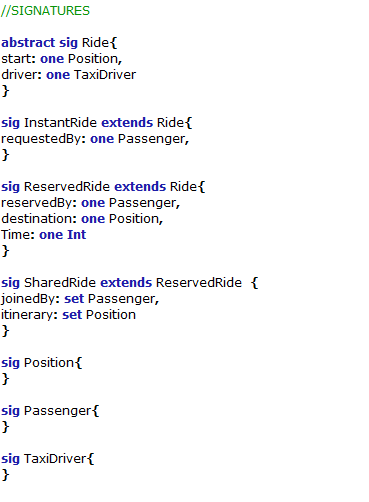
\includegraphics[height=0.75\textwidth]{Sig}
\end{figure}
\newpage

\subsubsection{Join a ride}
\begin {tabular} {|p{3cm}|p{10cm}|}
\hline
Goal & G5\\
\hline
Actor & Passenger\\
\hline
Entry conditions & User registered and logged in\\
\hline
Flow of events &
\begin {itemize}
\item The passenger clicks on join button
\item The passenger insert starting position and destination
\item The passenger choose the ride to join
\item The passenger clicks on confirm button
\end {itemize}\\
\hline
Exit conditions & The system add the passenger to the ride and send a notification to all passengers that joined the ride \\
\hline
Exceptions & Ride is already full, passenger has a ride that is occurring 30 minutes from the shared ride time \\
\hline
\end {tabular}
\begin{figure}[h!]
	\centering
	%	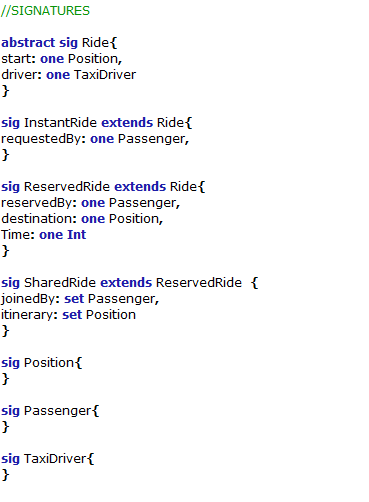
\includegraphics[height=0.75\textwidth]{Sig}
\end{figure}
\newpage

\subsubsection{Cancel a reservation/shared ride}
\begin {tabular} {|p{3cm}|p{10cm}|}
\hline
Goal & G6\\
\hline
Actor & Passenger\\
\hline
Entry conditions & User registered and logged in\\
\hline
Flow of events &
\begin {itemize}
\item The passenger clicks on cancel reservation button
\item The passenger clicks on confirm button
\end {itemize}\\
\hline
Exit conditions & The system cancels the reserved ride\\
\hline
Exceptions & Ride is occurring in 30 minutes, other users have already joined the ride \\
\hline
\end {tabular}
\begin{figure}[h!]
	\centering
	%	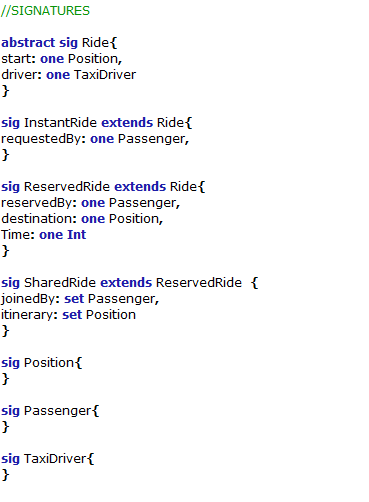
\includegraphics[height=0.75\textwidth]{Sig}
\end{figure}
\newpage

\subsubsection{Leave a shared ride}
\begin {tabular} {|p{3cm}|p{10cm}|}
\hline
Goal & G7\\
\hline
Actor & Passenger\\
\hline
Entry conditions & User registered and logged in\\
\hline
Flow of events &
\begin {itemize}
\item The passenger clicks on leave ride button
\item The passenger clicks on confirm button
\end {itemize}\\
\hline
Exit conditions & The system remove the passenger from the ride and send a notification to all passengers that joined the ride \\
\hline
Exceptions & Departure time is in fifteen minutes.\\
\hline
\end {tabular}
\begin{figure}[h!]
	\centering
	%	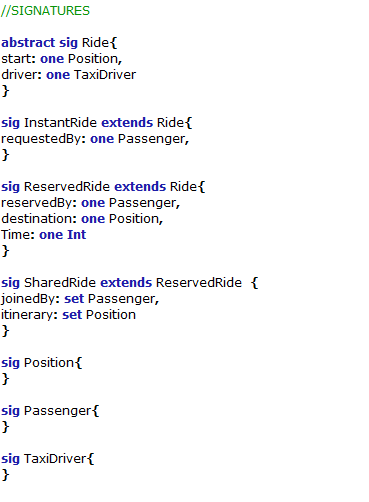
\includegraphics[height=0.75\textwidth]{Sig}
\end{figure}
\newpage

\subsubsection{Set availability}
\begin {tabular} {|p{3cm}|p{10cm}|}
\hline
Goal & G8\\
\hline
Actor & Driver\\
\hline
Entry conditions & User registered and logged in\\
\hline
Flow of events &
\begin {itemize}
\item The driver set his availability
\item The driver clicks on confirm button
\end {itemize}\\
\hline
Exit conditions & The system add the driver to the taxi's queue.\\
\hline
Exceptions & none \\
\hline
\end {tabular}
\begin{figure}[h!]
	\centering
	%	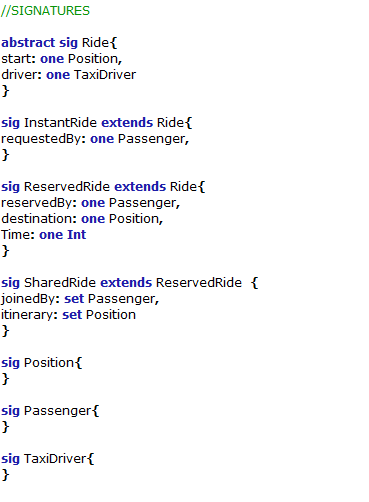
\includegraphics[height=0.75\textwidth]{Sig}
\end{figure}
\newpage

\subsubsection{Accept or refuse request}
\begin {tabular} {|p{3cm}|p{10cm}|}
\hline
Goal & G9\\
\hline
Actor & Driver\\
\hline
Entry conditions & User registered and logged in\\
\hline
Flow of events &
\begin {itemize}
\item The driver receive a call from the system
\item The driver accept or refuse it
\end {itemize}\\
\hline
Exit conditions & The system assign the driver to a ride\\
\hline
Exceptions & Driver doesn't answer in time\\
\hline
\end {tabular}
\begin{figure}[h!]
	\centering
	%	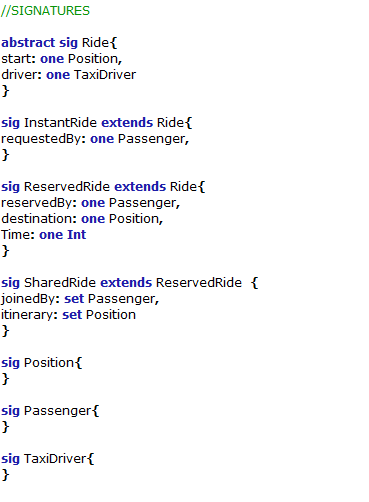
\includegraphics[height=0.75\textwidth]{Sig}
\end{figure}
\newpage

\subsection{Class Diagram}
\begin{figure}[h]
	\centering
	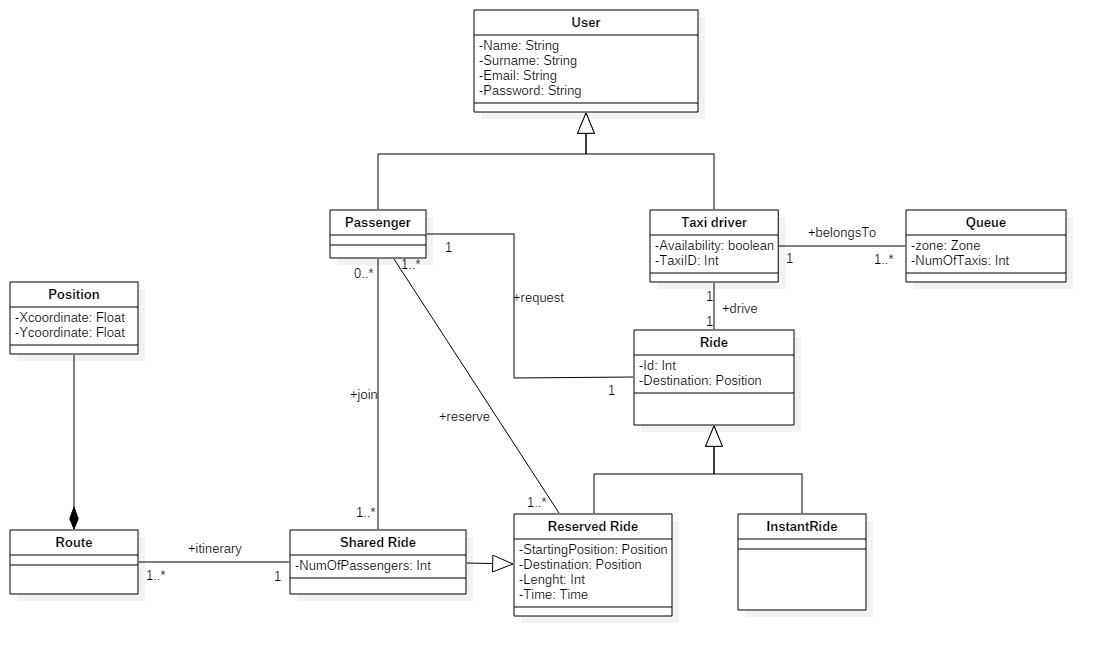
\includegraphics[width=\textwidth+]{class_diagram}
\end{figure}
\newpage
\subsection{State chart diagram}
\begin{enumerate}
	\item User makes a request
	\begin{figure}[h]
		\centering
		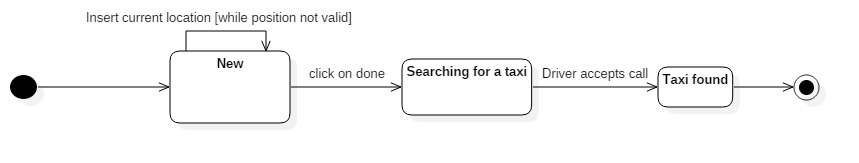
\includegraphics[width=\textwidth+]{Request}
	\end{figure}

	\item User makes a reservation
	\begin{figure}[h]
		\centering
		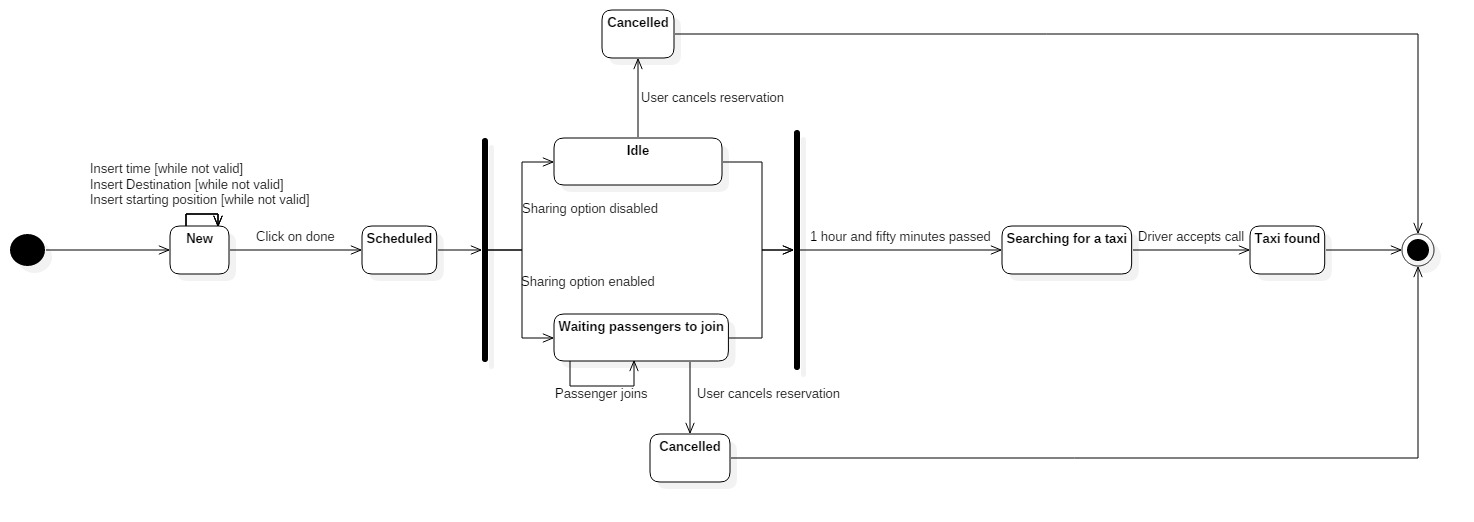
\includegraphics[width=\textwidth+]{reservation}
	\end{figure}
	\newpage
	\item Taxi driver states
	\begin{figure}[h]
		\centering
		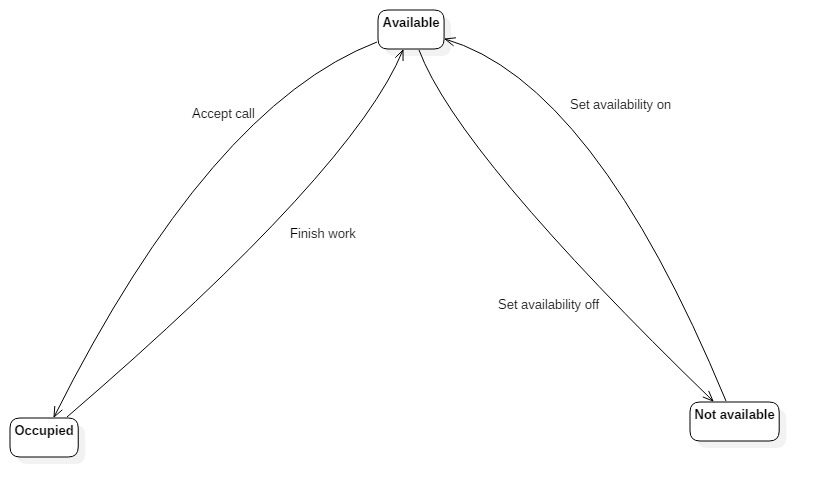
\includegraphics[width=\textwidth+]{taxidriver_statechart}
	\end{figure}
\end{enumerate}